\documentclass[prstpaper]{revtex4-2}
% word limit is 6000
%reprint,
%superscriptaddress,
%groupedaddress,
%unsortedaddress,
%runinaddress,
%frontmatterverbose, 
%preprint,
%preprintnumbers,
%nofootinbib,
%nobibnotes,
%bibnotes,
% amsmath,amssymb,
% aps,
%pra,
%prb,
%rmp,
%prstab,
%prstper,
%floatfix,
%]{article}
\usepackage{hyperref}
%\usepackage{times}
\hypersetup{}

%\usepackage{setspace} %for double-spacing submit version
%\doublespacing
\usepackage{amssymb}
\usepackage{adjustbox}
\usepackage{graphicx}% Include figure files
\usepackage{dcolumn}% Align table columns on decimal point
\usepackage{svg}
\usepackage{biblatex}
\usepackage{bm}
\usepackage{amsmath}
\DeclareMathOperator*{\argmax}{arg\,max}
\DeclareMathOperator*{\argmin}{arg\,min}
\usepackage{lipsum,framed}
\usepackage[mathlines]{lineno}% Enable numbering of text and display math
%\linenumbers\relax % Commence numbering lines
\usepackage{mathtools}
%\usepackage{biblatex}

%\addbibresource{export.bib}
\usepackage[left=2.5cm,top=3cm,right=2.5cm,bottom=3cm,bindingoffset=0.5cm]{geometry}
%\usepackage{texcount}
\begin{document}

%\preprint{APS/123-QED}

\title{Radial Control of Pathogens Invading Spatially Structured Multi-Species Populations}% Force line breaks with \\

\author{Alexis Vargas Richards (ar2185@cam.ac.uk)}
\affiliation{Girton College, Supervisor Prof NJ Cunniffe}

\maketitle

\section*{abstract}
Plant disease imposes a significant health, economic, and social burdens across the world. The impact of the responsible phytopathogens can often be reduced by control measures. However, phytopathogens may infect and transmit between more than one species of host, and can behave differently in each host species. This may pose a challenge for disease control. We formulate models for an invading disease subject to periodic survey-based detection and removal of hosts within a control radius or radii, and characterise where and how radial control breaks down. Our parameterisation is inspired by the emerging phytopathogen \emph{Xylella fastidiosa}, which infects multiple host species.

We find that for unclustered and clustered landscapes, a small proportion of cryptic hosts leads to a nonlinear breakdown in single-radius control in a subset of parameterisations. This is modulated in significant ways by the patterning of the hosts as well as asymmetric transmission.

\newpage
%\tableofcontents
\section*{INTRODUCTION}

Epidemics of plant disease have occurred throughout history. They can cause significant damage, including to economies and ecosystems alike \cite{Boyd2013}. However, how best to control invading plant disease is not a trivial question \cite{}. The control problem becomes less tractable when cryptically infected hosts are present, and epidemiological parameters are uncertain \cite{Cunniffe2015}, as is likely to be the case in real-world diseases and periodic surveying.
Current literature has not thoroughly addressed the interplay between host heterogeneity, patterning in space and disease controllability in a radial control programme context. Modelling multi-host pathogens have been highlighted as a key challenge in disease ecology \cite{Buhnerkempe2015}, and multiple current important pathogens infect more than one species \cite{Heesterbeek2007} \cite{}. Existing work on asymmetric transmission has been motivated by diseases such as \emph{Phytophthora ramorum}, etiologic agent of sudden oak death (SOD). \emph{Xylella fastidiosa} is another emerging multi-host pathogen causing severe economic losses in Europe \cite{Bodino2021} \cite{Martelli2016}. It is projected to continue to cause future economic damage (up to the order of billions of euros) to olive production over the next 50 years, since it causes Olive Quick Decline Syndrome (OQDS) \cite{Schneider2020}. It is also responsible for several other diseases of major agricultural importance, Pierce's disease of grapevine and almond leaf scorch (ALS) \cite{GimenezRomero2024}\cite{Gibin2023}. Current EU legislation recommends the removal of all hosts within a radius of 100 m of a detected infection \footnote{https://planthealthportal.defra.gov.uk/pests-and-diseases/high-profile-pests-and-diseases/xylella/}. Such radial removal following periodic surveying is a common and tractable disease control regime, with some computational literature investigating \cite{Cunniffe2015} \cite{HyattTwynam2017} \cite{Jerome2021} \cite{Parnell2009} \cite{Parnell2010}.


However, the invasive bacterium \emph{X. fastidiosa} is also notable for its extremely broad host range \cite{Gibin2023}. Radial control programmes for disease control have been known to fail in the past \cite{}. Further, the implications of host heterogeneities for disease dynamics in the case of animal pathogens 
The design of control programmes for infectious diseases of animals 
.Pathogens such as \emph{X. fastidiosa} which can infect multiple host species \cite{Gibin2023} result in multiple tunable control parameters: $r_{i}$, the removal radius for a host of species $i$. The case where $r_{i}$ are different represents a use of readily obtainable epidemiological information even in remote or resource-poor settings: host species is easily identifiable, whereas broader knowledge of factors such as local host density may not be. This motivates the investigation of potential benefits of two-radius control.

Misspecification of epidemiological parameters is relatively common, and therefore this work also aims to study the degradation (if any) of strategies to control invasive infectious disease under partially characterised parameters, as elucidated briefly in \cite{HyattTwynham2017} for a single host type system. Existing work on the impact of landscape structure on phytopathogen control includes \cite{Parnell2009} \cite{Parnell2010}, where Asiatic citrus canker was used to test the effect of clustering and host density in single-species landscapes. Recent work has introduced the O-ring statistic for use in spatial disease analysis \cite{}, and this is used to obtain expressi. In both of these cases, the host density and clustering was observed to alter the optimal radius of host removal. Here, observation of different host density regimes is made in an attempt to recapitulate the potential for divergent disease control dynamics in different field settings. 

Hence, this work aims to address several largely unanswered questions, with particular relevance to the efficacy of control of invading \emph{X. fastidiosa} in complex areas on a small scale, from an external source of inoculum. 

\begin{framed}
\subsection*{Key Questions}

\begin{description}

   \item[Q1] {How does varying the proportion of species A (less cryptic) and species B (more cryptic) affect control efficacy? What is the divergence between an approach optimised to each landscape case, versus a control strategy optimised to a single host type landscape? }
    \item[Q2] {Are there nonlinearities in the breakdown of control as landscape or host parameters change? Are these present in both the parameter misspecification case and the landscape-optimised case?}
    \item[Q3] {Is having species-specific control radii a significantly better-performing strategy than constant control radius?}
    \item[Q4] {Does the nature of increased crypticity (i.e., either lower detection probability or longer cryptic period) make a difference to disease controllability? }
    \item[Q5] {How does asymmetric transmission affect the efficacy of control?}
    \item[Q6] {How do different host landscapes modulate the above effects?}
\end{description}
\end{framed}

\section*{METHODS}
\subsection*{Simulating Host Landscapes}


Epidemics on the following host landscapes were examined:

\begin{itemize}
\item[\textbf{LAN1}] Complete Spatial Randomness (CSR) 
\newline
\label{LAN1}
    Hosts are distributed according to random floats generated with uniform probability on the [0,1] interval, and scaled by length $L$ as necessary to a square. The probability distribution for position of each point is independent and identically distributed. 
    
\item[\textbf{LAN2}]  Neyman-Scott Process \label{LAN2}
\newline
    The Neyman-Scott process simulates a clustered distribution of points \cite{vandenBosch2024}. The function \texttt{rCauchy} from package \texttt{spatstat} \cite{Baddeley2015} was used to generate Neyman-Scott landscapes in R version 4.4.2 \cite{RCoreTeam}, using a custom script, with each host type generated separately and combined into a single multi-type point process. Since the number of points in the point pattern generated for each host type could not be explicitly specified, a condition-based error threshold was imposed: if the number of generated points was 
    \end{itemize}

\subsection*{Single-Type Epidemic Model}

The model is a spatial, stochastic Susceptible-Cryptic-Infected-Removed (SCIR) model, following \cite{HyattTwynam2017} for the single host-type case. It is an individual-based model (IBM):  the position of each host and its infection status is tracked during the time course of a simulated epidemic.

%\begin{figure}
%%\includesvg[scale=.5]{deterministic_singlesps_calib.svg}% Here is how to import EPS art
%\caption{\label{fig1} Deterministic SCIR Dynamics in The Absence of Control or Spatial Detail, under Default Parameterisation %%from \cite{HyattTwynham2017}. The cryptic 
%Normalised for 1/2 hosts infected at 500 days.}. 
%\end{figure}

%\begin{figure}%
%\includesvg[scale=.5]{stoch_det.svg} 
%\caption{\label{fig2} Stochastic and Deterministic Models Correspond: No Control Implemented. Stochastic epidemics are indicated by translucent lines; the corresponding deterministic epidemic is solid. Parameters as in
%\hyperref[fig1]{FIG 1.}.}
%\end{figure}


%\begin{figure}
%%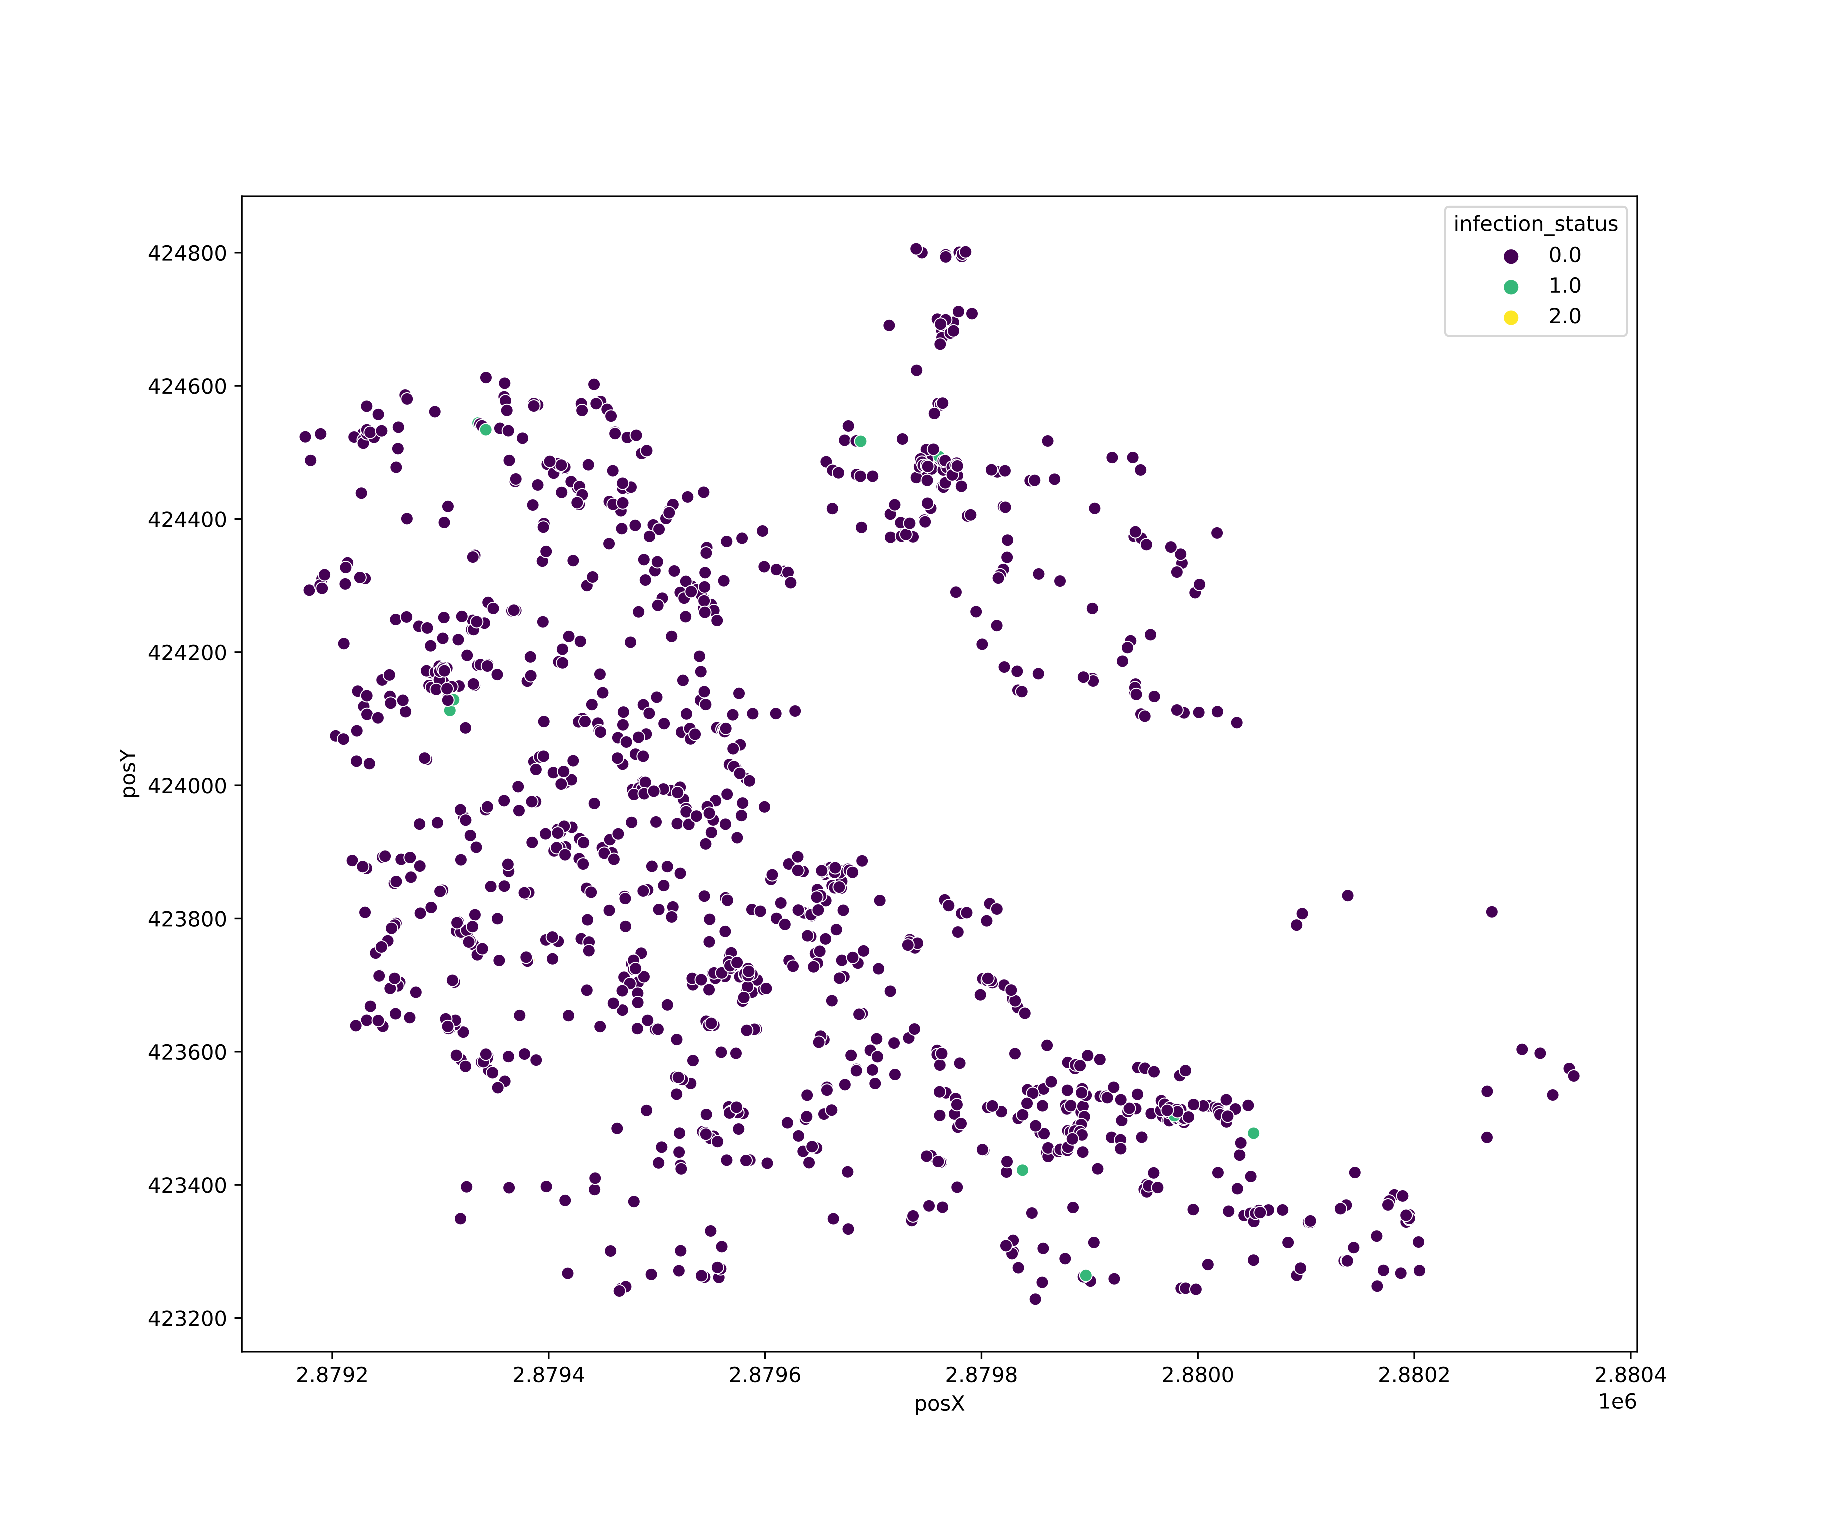
\includegraphics[scale=.5]{fig2}
%\caption{\label{fig} Spatially Explicit Spread on the Miami Citrus B2 Dataset. The area of the B2 survey was approximately $15.5km^2$, and there are approximately 1100 hosts (citrus trees) present. \cite{Gottwald2002}} 
%\end{figure} 

The population size is $N$ and is constant. Hosts may move between the following compartments: $S$, $C$, $I$ and $R$.

\begin{equation}
	S(t) + C(t) + I(t) + R(t) = N(t) = N,   \forall t \ge 0 
\end{equation}

At time $t = 0$, $C_0$ hosts are randomly infected. The $C_{0}$ hosts are cryptic: they do not show symptoms but may transmit infection to other hosts. A preexisting control programme involves surveys of the host population at a frequency every $\Delta$ days, and that a symptomatically infected host of species $i$ is detected with probability $p_i$. The time of the first control event, $\Delta_{0}$, is randomly selected from the  $[0, \Delta]$ interval, to reflect an ongoing 'preventative control' programme aimed at preventing the incursion of invasive plant disease, and the unpredictability of when an incursion of pathogenic material may occur. To reflect the complexity of real-world control, if the host is cryptically infected the infection is detected with probability 0, and with $p_{d, i}$ for host of type $i$ in compartment I (symptomatic infected hosts), and this is species-specific. The number of hosts of each species detected during a round of control is drawn from a binomial distribution.

If detected, the host is removed, along with any host within a radius of $r_{i}$ m. of the removed host, for a host of species $i$. Often, the radius is the same for both species, $r_{A} = r_{B} = r$.
The single-species model with single-radius control corresponds exactly to the case of constant-radius control examined in \cite{HyattTwynam2017}, where there is a single parameter $r$ which may be optimised for disease control.

\subsection*{Multitype Epidemic Model}

To reflect the complexity of \emph{Xylella fastidiosa}, the model was extended to a multi-type model with two host types, denoted as A and B respectively. In the single-type case, transmission parameterised directly by only one parameter, $\beta$. However, since the pathogen can infect two host types, there is an increased set of parameters in the two-species case. In particular, the transmission of infectious propagules from species A $\rightarrow$ B may occur with a different propensity than B $\rightarrow$ A, or A $\rightarrow $A, in the most general case. One way to parameterise the potentially asymmetric transmission is as in \cite{NdeffoMbah2010}, where the transmission matrix is 

\begin{equation}
\label{ndeffo}
\bf{T_{mat}} = 
\begin{pmatrix}
\beta_{11} & \beta_{12} \\
\beta_{21} & \beta_{22}
\end{pmatrix} 
\end{equation}

with $\beta_{ij}$ the transmission parameter from species $i \rightarrow j$. This constitutes a phenomenological approach, but for the below model, we adopt a slightly different parameterisation which is more biologically inspired but not mathematically distinct from Eq. (\ref{ndeffo}). (It depends on the assumption that all propagules behave the same, irrespective of the host species releasing them.) 

The constant parameterising transmission from individuals of species $i$ to $j$, $\beta_{ij}$, is a product of both the infectivity of the $i$ species ($\nu_{i}$, the susceptibility to infection of the $j$ species $\phi_{j}$, and the permissivity of the environment to the infectious agent $\eta$. Hence, we write

\begin{equation}
\beta_{ij} = \nu_{i} \phi_{j} \eta
\end{equation}

and for $j \rightarrow i$:

\begin{equation}
\beta_{ji}= \nu_{j} \phi_{i} \eta
\end{equation}

We note that in the general case $\beta_{ij} \neq \beta_{ji}$ (asymmetric transmission).

\begin{equation}
    \begin{pmatrix}
\beta_{11} & \beta_{12} \\
\beta_{21} & \beta_{22}
 
\end{pmatrix} = 
\begin{pmatrix}
\nu_{1} \phi_{1} \eta & \nu_{1} \phi_{2} \eta \\
\nu_{2} \phi_{1} \eta & \nu_{2} \phi_{2} \eta \\
\end{pmatrix}
\end{equation}

$\eta$ reflects the fraction of infectious propagules that - having been released by a primary host - go on to physically reach a potential secondary host. $\eta$ is a function of environmental conditions, but we assume it is equal for all scenarios here and thus remove it: 

\begin{equation}
\label{nuphi}
   \bf{T_{mat}} = 
\begin{pmatrix}
\nu_{1} \phi_{1} & \nu_{1} \phi_{2} \\
\nu_{2} \phi_{1} & \nu_{2} \phi_{2} \\
\end{pmatrix}
\end{equation}

We also incorporate species-specific crypticity, since different species are likely to manifest symptoms at different times after infection (relevant to $\sigma$) and potentially to different extents (relevant to probability of detection, $p_d$). 

\begin{equation}
   \bf{S_{mat}} = 
\begin{pmatrix}
\sigma_{1} & \sigma_{2} \\
p_{d_{1}} & p_{d_{2}}\\
\end{pmatrix}
\end{equation}

The stochastic dynamics in the absence of control are governed by the following equations for transition rates for each individual which are:

%\end{eqnarray}array}
\label{twospecies}
    
%\end{equation}
\begin{eqnarray}    
Rate \left( S_{1} \rightarrow C_{1}\right) &=& \phi_{1} \left( \nu_{1} \sum_{i \in C_{1}(t), I_{1}(t)}^{} K(d_{ij}; \alpha) + \nu_{2} \sum_{i \in C_{2}(t), I_{2}(t)}^{} K(d_{ij}; \alpha) \right) \\
   Rate \left( C_{1} \rightarrow I_{1}\right)  &=&  \sigma_{1} \\
%\label{twospeciesB}
    Rate \left( S_{2} \rightarrow C_{2}\right) &=& \phi_{2} \left( \nu_{1} \sum_{i \in C_{1}(t), I_{1}(t)}^{} K(d_{ij}; \alpha) + \nu_{2} \sum_{i \in C_{2}(t), I_{2}(t)}^{} K(d_{ij}; \alpha) \right) \\
   Rate \left( C_{2} \rightarrow I_{2}\right) &=&  \sigma_{2} \\
\end{eqnarray}

and $I(t) = N(t) - (S(t) + C(t))$ since there is no control and no host death, $\gamma = 0$. In this special case, $K(d_{ij}; \alpha) = 1$ for all hosts. Space is considered only in the stochastic model.

For the spatial stochastic model,  two potential kernel functions are the thick-tailed Cauchy kernel and the thin-tailed exponential kernel, which have the forms given in \cite{HyattTwynham2017}. Both of these functions are parameterised by the dispersal scale $\alpha$, although the Cauchy kernel gives a higher probability of long-distance dispersal events than the exponential kernel.
The system is simulated stochastically using Gillespie's Direct Simulation Algorithm as outlined in \cite{Keeling2008}. When a timestep would cause the time (measured in days) to exceed that of a scheduled control survey and possible host removals, the control event would be performed first and the time set to the scheduled control time. Transition rates for the hosts were then recomputed and the time-step recalculated.  

\subsection{Parameterisation from \emph{Xylella} studies}

The model formulated here is not, and does not aim to be, predictive. However, efforts have been made to place parameter values within biotic ranges so that the qualitative dynamics of the control problem can be examined. 

\subsubsection{Crypticity Parameters: $p_{d}$ and $\sigma$}

$p_{d}$ is a function of the surveying method and the equipment used, and therefore this parameter has been assigned to a range of values. However, for the other crypticity-determining parameter, $\sigma$, EFSA provide several species-specific estimates in \cite{Bragard2019}. Specifically, the estimated mean asymptomatic time is $\frac{1}{452}$ days$^{-1}$ for \emph{Olea europea} infected by \emph{X. fastidiosa subsp. pauca}. However, the estimated median asymptomatic time via parametric and non-parametric methods respectively given in \cite{Bragard2019} lead to estimates of $\frac{1}{203}$ and $\frac{1}{452}$ days$^{-1}$ for the asymptomatic period. An additional complexity is that the SCIR model assumes that hosts are instantaneously infectious to others following infection, but this is not realistic \cite{Leclerc2014}. Instead, there is a non-zero incubation time, not modelled here. In view of the considerable uncertainty on precise quantification and in addition the simplistic nature of exponentially distributed residence time in the Cryptic compartment, $\sigma$ is set to $\frac{1}{350}$  days$^{-1}$., but senstivity analysis will be performed.

\subsubsection{Dispersal Kernel and Scale Parameter of \emph{Xylella fastidiosa}}

In \cite{White2017}, a grid-based approach (in contrast to the present model) was used to model and predict the early spread of \emph{X. fastidiosa} in Apulia, Italy. Dispersal in that case was argued to be stratified, with long-distance dispersal events occurring. Hence, two separate dispersal mechanisms were incorporated, an exponential kernel to model shorter dispersal events, parameterised by $\alpha = 100 m$, and a longer-range dispersal generator (2D Gaussian). A simpler approach taken here is the use of the thicker-tailed Cauchy dispersal kernel, in combination with the thinner-tailed exponential kernel which is $K_{\exp}(d; \alpha) = \exp\left(\frac{-d}{\alpha}\right)$ as in \cite{HyattTwynham2017}. 

\emph{Xylella fastidiosa} is vectored in the European Union (EU) by the spittlebug \emph{Philaenus spumarius} \cite{Bragard2019}\cite{Bodino2021}. Mark-release-recapture (MRR) provides quantification of the rates of dispersal of the vectors - and therefore the pathogen - through time. MRR was used in \cite{Bodino2021} to estimate a Gaussian dispersal kernel at different times following vector release. 50\% of spittlebugs stayed within 200m over the course of 6 months in an olive grove setting in Apulia, Italy. Using the cumulative distribution function formula (CDF) for a 2D normalised exponential dispersal kernel, this median value implied a scale parameter of 119m for the exponential kernel.
Since the Cauchy kernel $K(d_{ij}; \alpha) = \frac{1}{1+\left(\frac{d_{ij}} {\alpha}\right)^2}$ cannot be normalised in $\mathbb{R}^2$, the scale parameter for this kernel was derived via least-squares fitting to the exponential kernel ($\alpha_{expon.}=119$m), giving a scale parameter for the Cauchy kernel of $\alpha_{cauchy}= 84.5$m.

In the short range eco-epidemiological model\cite{Bragard2019}, the susceptibility of the host plant was  defined by \cite{Bragard2019} as  the average probability a host is systemically infected following 1 day of feeding by an infected vector. 

Hence, for experiments examining solely the effect of crypticity, the value of $\phi_{i}$ \footnote{This corresponds closely to $\phi_{i}$, susceptibility of species $i$ in \ref{nuphi}.} was set to to equal irrespective of host type. This also enabled varying the proportion of host type B without repeated normalisation. However, for investigations of asymmetric transmission this could not be avoided.

\subsection{Normalisation and Epidemic Termination Condition}
Landscape structure and host density influence disease dynamics (and therefore control) \cite{Parnell2010} \cite{Jerome2021} \cite{Parnell2009}. 
For the following results, it is important to note that the termination condition is: $S(t) = 0$ or $C(t) + I(t) = 0$. Epidemic impact, $K_{E}$ is computed as 

\begin{equation}
    K_{E} = C(t) + I(t) + R(t)
\end{equation}

once $C(t) + I(t) = 0 $ or $ S(t) = 0$. 

\begin{table}
\centering
\begin{adjustbox}{width=\textwidth}
\small
    \begin{tabular}{|c|c|c|c|c|}
    \hline
         \textbf{Host Type Identity (if appl.)}  & \textbf{Parameter Description} & \textbf{Parameter Symbol} & \textbf{Values} & \textbf{Source}\\
         \hline
        \hline
         \emph{O. europea} infec. \emph{X.f. subsp. pauca} & Symptom appearance rate & $\sigma$& $\frac{1}{350}$ $day^{-1}$ &  \cite{Bragard2019}\\
        \hline
         \emph{O. europea} & Death rate (I) & $\gamma$  & 0.00053 day$^{-1}$&  \cite{Bragard2019} \\
        \hline
        Generic & Susceptibility to infection& $\phi$& 0.09 or 0.14 & \cite{HyattTwynham2017}\\
        \hline
        Generic & Infectivity & $\nu$ & fit via normalisation & N/A \\
        \hline
        \emph{X. fastidiosa subsp. pauca}& Exponential Kernel Scale Parameter & $\alpha_{exp}$ & 119 m & Median fit to \cite{Bodino2021}\\
        \hline
        \emph{X. fastidiosa subsp. pauca}& Cauchy Kernel Scale Parameter & $\alpha_{cauchy}$ & 84.5 m & Least-squares fit to $\alpha_{exp}$ \\
        \hline
    \end{tabular}
    \end{adjustbox}
    \caption{Parameter values and sources used for this study: Host Demography and Infection Processes. See body text for details of fitting performed.}
    \label{tab:my_label}
\end{table}



\begin{table}
    \centering
    \begin{tabular}{|c|c|c|c|c|}
    \hline
        \textbf{Species Identity}  & \textbf{Parameter Description} & \textbf{Parameter Symbol} & \textbf{Values} & \textbf{Source} \\
        \hline \hline
        e.g., Olive & $\mathbb{P} \mathrm{(detected | surveyed)}$& $p_{d;A}$& 1 & \cite{Bragard2019} \\   
        \hline
         Cryptic Host & $\mathbb{P} \mathrm{(detected | surveyed)}$& $p_{d;B}$& 0.2 - 1& None\\        
        \hline
         N/A & First survey time & $\Delta_{0}$& Rand*[0,90] & None\\
        \hline
        N/A & Survey frequency & $\Delta$ & 90 days$^{-1}$&  \cite{HyattTwynham2017}\\
        \hline
         Olive-like & Fraction surveyed (A)  & $F_{A}$ & 1 &  \cite{HyattTwynham2017}\\
        \hline
         Cryptic host & Fraction surveyed (B) & $F_{B}$ & 1 & \cite{HyattTwynham2017}\\
        \hline
    \end{tabular}
    \caption{Parameter values and sources used for this study: Radial Control Processes}
    \label{tab:my_label}
\end{table}
\subsection{Landscape Parameterisations and Landscape Simulation}

Survey data for the geo-referenced location of potential hosts of \emph{X. fastidiosa subsp. pauca} in Puglia, Italy 2022 was  used to parameterise host landscapes. \footnote{Available at: http://www.emergenzaxylella.it/portal/portale\_gestione\_agricoltura/Download/mon\_pauca.} 

The \emph{Xylella} host data were therefore transformed to a UTM coordinate system using the R package 'sf' \cite{}. This was input as a multi-type point pattern to \texttt{spatstat}, with the window of observation automatically inferred using the Ripley-Rasson method \cite{Ripley1977}. Duplicated points were removed, and species with frequency $< 0.1$ were also excluded to reduce the number of types in the multitype point process.  
In all cases, the total number of hosts in the model, $N$, was set at 1110 to upper bound computation time, and approximately follow \cite{HyattTwynam2017}. For each landscape parameterisation, 5 landscape instances were generated, with 50 epidemics performed on each instance giving 250 replicates for each generative landscape parameterisation.

\begin{table}
    \centering
    \begin{tabular}{|c|c|c|c|c|}
    \hline
        \textbf{Landscape Model} & \textbf{Parameter Description} & \textbf{Parameter Symbol}
        & \textbf{Values} & \textbf{Source}\\
        \hline \hline
        CSR: Low Density Regime & &  & 69 hosts /km$^2$,  & \\
        \hline
        CSR: Medium Density Regime & Landscape Area & $L^{2}$ & $3.5 $x$ 3.5 $km$12.25$km$^2$,  & \\
        \hline

        \end{tabular}
    \caption{Parameter values and sources used for this study: Landscapes}
    \label{tab:my_label}
\end{table}
\subsection*{Parameter Scans: Adapted and Misspecified Control and Epidemic Outcome Metrics}

For each landscape considered, the radius of host removal was varied on an interval of [0,100] to find the approximate optimal radius of removal, $r_{rem}^{*}$ with respect to Median ${K_{E}}$. Additional epidemic outcome metrics were Area Under the Disease Progress Curve (AUDPC) \cite{Cunniffe2015} and the epidemic impact per host type.
In 2-dimensional parameter sweeps, the parameter range with 250 replicates per point. Computation of an approximately optimal control strategy for each set of landscape parameters was performed  by sweeping radius value for each landscape parameterisation, and identifying the radius $\hat{r_{opt}}$ giving the lowest median epidemic impact.
In both cases above, the free parameters for optimisation were the radius of removal $r_{removal}$ or two species-specific radii of removal, $r_{A}$ and $r_{B}$ for the one- and two-radius cases respectively. 



\section*{RESULTS}



%\begin{figure}

%\includesvg[scale=0.5]{almond.svg}
%\includesvg[scale=0.5]{olive.svg}
%%\includegraphics[scale=0.5]{Rplot01.eps}
%\caption{\label{fig} The Distribution of Almond and Olive Trees Overlap. Local density of the hosts varies significantly. }
%\end{figure}


\begin{figure}[hbt!]
\includesvg[scale=0.45]{epidemics.svg}
%\includesvg[scale=0.5]{olive.svg}
%%\includegraphics[scale=0.5]{Rplot01.eps}
\caption{ \label{epi_nocontrol} Progression of an uncontrolled epidemic on a host landscape of complete spatial randomness, where half of hosts are of type B. Approximately half the hosts are infected by 500d., and host deaths begin to be significant towards T = 750 days. Parameterisation is $\emph{Xylella}$-like (see Methods). Host density $\approx$ 123 hosts km$^{-2}$, and N = 1110. }
\end{figure}


In Fig. \ref{epi_nocontrol} the uncontrolled epidemic parameterised for \emph{Xylella} qualitatively exhibits approximately wave-like infection fronts expanding from the multiple initial sites of infection.

\subsection*{Effect of Crypticity Parameters on Control in the Single-Type Case}

For a thick-tailed Cauchy kernel, simply varying $p_d$ on [0, 1] with control optimised perturbs mean epidemic impact as follows: 

\begin{figure} [hbt!]
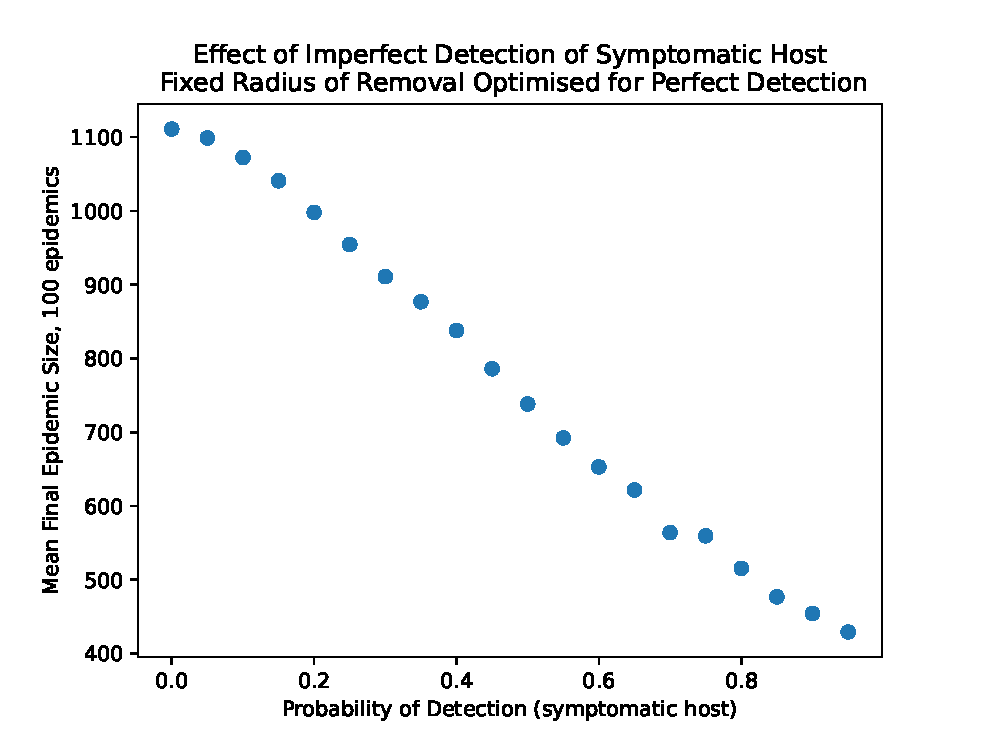
\includegraphics[scale=.4]{pd.eps}
%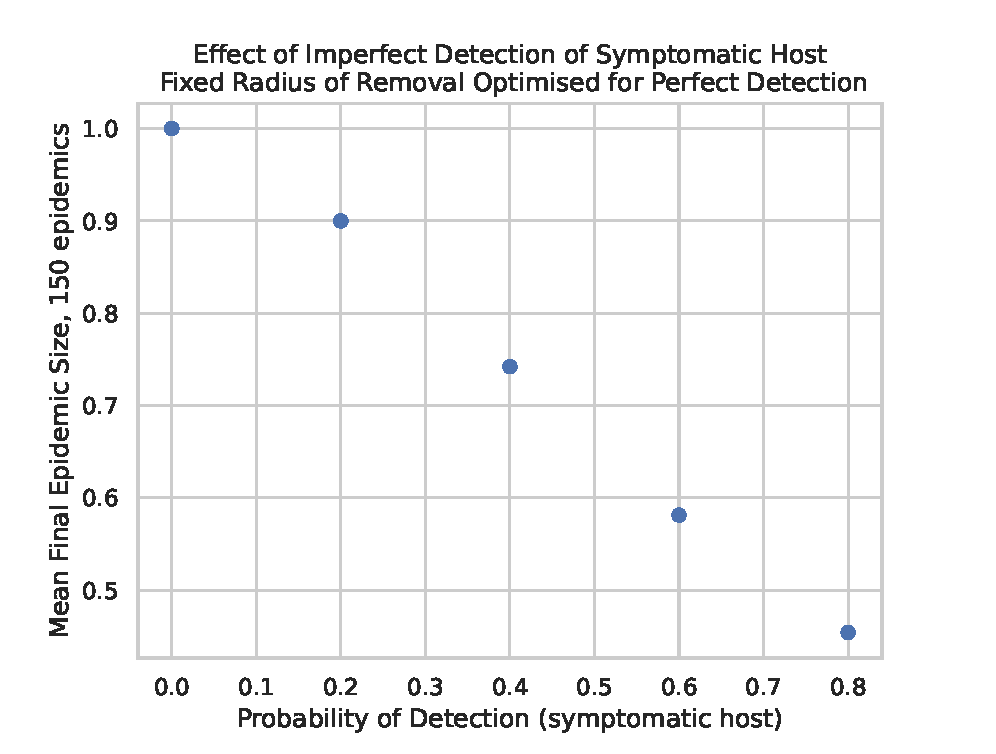
\includegraphics[scale=1]{detection_sweep.eps}
\caption{\label{fig} Misspecification of detection probability causes approximately linear decay in control efficacy for the Cauchy kernel as quantified by $K_E$. Parameters as in \cite{HyattTwynham2017}. }
\end{figure}

This approximately linear increase in epidemic impact, $K_{E}$, corresponds to a misspecification of the detection probability parameter. This is plausible. Hence, the efficacy of constant radius of removal control does not exhibit abrupt nonlinearities if $p_{d}$ is incorrectly assumed to be 1, at least for the parameters and kernels chosen. This is as expected from the governing equations for the system \ref{}.  

%\begin{figure}
%\includesvg[scale=0.8]{2d_draft_sweep.svg}
%\caption{\label{fig} Radial control performs differently across different probabilities of detection, in the Citrus Landscape. Optimal radius of removal is landscape dependent.}
%\end{figure}

Other parameters may also be misspecified. Specifically, $\sigma$, which parameterises residence time in the Cryptic compartment, may be misspecified. Assuming control is optimised for the nominal value of $\sigma =  $, then the expected final size varies as in 

%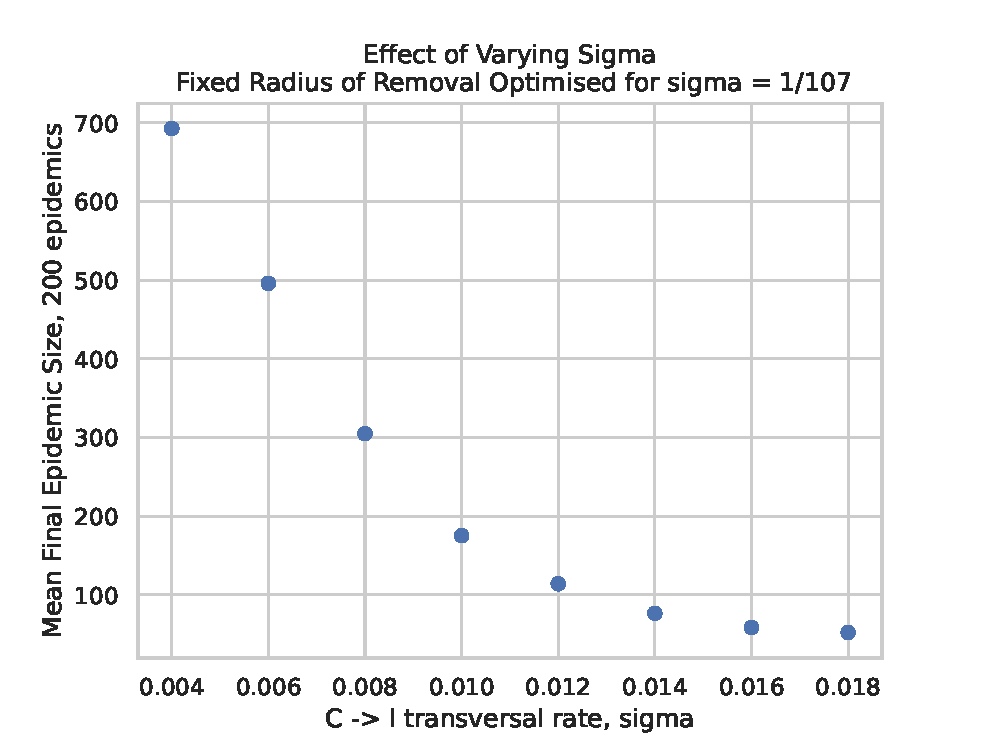
\includegraphics[scale=1]{sigma_sweep.eps}

This is as expected given that the expected residence time in the cryptic compartment is $\frac{1}{\sigma}$.

Simultaneous misspecification of the two parameters is also a case which may occur in real-world conditions. \cite{HyattTwynham2017} considered the case of misspecification of $\sigma$, $p_{d}$ and found a linear change in control efficacy. 


\subsection*{Control in a Landscape of Complete Spatial Randomness}

The simplest model for the two-species distribution is complete spatial randomness (CSR), a homogeneous Poisson point process. The two species are distributed uniformly on a square domain of length $L$ and area $L^2$. One species is a more cryptic host and the other is more symptomatic. Survey frequency is fixed at $\Delta = 90$ days. Control may either use a fixed radius of removal, irrespective of the species being removed, or alternatively species-specific removal radii are used (see Key Questions box). 

We compare the species-specific removal radius case to the simpler case where there is only one parameter that can be optimised, $r_{\mathrm{removal}}$ - i.e., the same management strategy is used for both species. 

\begin{figure}[hbt!]
\includesvg[scale=0.6]{csr_4k_deltapd_exp.svg}
\caption{\label{csr4kdeltapd} The effect of increasing the proportion of host type B, with $p_{d,B}  = 0.2 $ and $\sigma_{A} = \sigma_{B} = \frac{1}{350}  \mathrm{days}^{-1}$, on epidemic metrics for host landscapes of complete spatial randomness with $\approx 70  \mathrm{ hosts} / \mathrm{km}^2$. \textbf{A)} The optimal radius of host removal generally increases as the proportion of cryptic hosts rises when measuring the Median epidemic impact $K_E$. \textbf{B)} The same epidemics as for \textbf{A)}, but AUDPC computed as the dependent variable. Near-Optimal AUDPC is attainable for a far broader range of control radii than optimal $K_E$.  
Optimal radii show a less pronounced trend with a smaller impact on Median AUDPC. Each block is 250 replicates at a resolution of 50 m.}
\end{figure}

\begin{figure}[hbt!]
%\includesvg[scale=.85]{4k_exp_csr_deltapd_misspecified.svg}
\includesvg[scale=0.85]{delta_compare_exp_csr_4k.svg}
\caption{\label{} Both landscape-optimised (with respect to $K_{E}$) and misspecified controls degrade in effectiveness as the proportion of cryptic hosts rises. \textbf{(A)} shows the close similarity in control efficacy as measured by $K_E$ as the fraction of host type B increases. \textbf{(B)}: The increase in AUDPC is more pronounced for the misspecified control case, and exhibits significant divergence away from landscape-adapted control as shown by the lack of overlap in interquartile ranges for Frac(B) $>$ 0.5. Epidemic data from Fig \ref{csr4kdeltapd}. [Note that x-jitter has been applied to prevent bar overlap in the x-direction.]}
\end{figure}

\begin{figure}[hbt!]
\includesvg[scale=0.65]{sigma_4000_csr_sym.svg}
\caption{\label{sigma4kcsrsym} \textbf{(A)} In the case where host type B has $\sigma_B$ = $\frac{1}{500}$ days$^{-1}$ but $p_{d,B} = 1$, optimal radius shows a less pronounced increase as Frac(B) $\rightarrow$ 1 than for the $\Delta p_{d}$  case (Fig. \ref{csr4kdeltapd}), increasing only slightly even as frac(B) $\rightarrow$ 1. \textbf{(B)} optimal radius of removal with respect to AUDPC shows no clear trend. Host density $\approx$ 70 hosts km$^{-2}$. }
\end{figure}

\begin{figure}[hbt!]
\includesvg[scale=0.85]{delta_sigma_4k_csr.svg}
\caption{\label{compare_strategies_delta_sigma} Performance of optimal-misspecified controls for the  case where $\sigma_{B} = \frac{1}{500} \mathrm{days}^{-1}$. \textbf{(A)} Close correspondence between the misspecified and optimal control strategies persists even as $\mathrm{Frac(B)} \rightarrow 1$ when measuring $K_{E}$.  \textbf{(B)} With AUDPC as the response variable, there is significant divergence between the two strategies, even for the mostly homogeneous landscapes, with $\mathrm{Frac(B)}$ small.}
\end{figure}



\subsection{Misspecified Control in Well-Mixed Landscapes: Control Efficacy Decays Under Increasing Proportion of Cryptic Hosts}

In the case of control optimised to a single host type, and a cryptic host having a low probability of being detected ($p_{d} << 1$) , then radial control becomes increasingly ineffective. However, the rate of increase in epidemic impact ($K_{E}$) and AUDPC shows qualitative differences to the case where 

Varying the proportion of species B on [0,1] with a constant radius of removal (31 m), gave the following results FIG \ref{fig5}.

\begin{figure}
\includesvg[scale=0.9]{prop_B_JAN.svg}
\caption{\label{fig5} Emergent nonlinearity in decaying efficacy of control as proportion of Cryptic species increases. The dispersal kernel is Citrus canker-like. Landscape of complete spatial randomness: 16km$^2$, 1200 hosts. $p_{d}  = 0.2$ for cryptic species (B) and $p_d$ = 1 for species A. Fixed radius of removal, 31 m. Cauchy kernel, $\alpha = 36.1$m}
\end{figure}

The decay of control efficacy is significantly faster than linear (as proportion(B) $\rightarrow$ 1 if the control is optimised only for the absence of the more cryptic B species. Hence, if host types are well-mixed and distributed randomly, then even the presence of a small fraction of very cryptic ($p_d$ = 0.2) hosts results in significantly damaged control (less than half of the population is spared). 

If, alternatively, the more cryptic B species had similar, high $p_{d}$, but instead a longer cryptic period as parameterised by $\frac{1}{\sigma}$, the control efficacy exhibits the following characteristic:

Export of infectious material to areas outside the modelled square domain is a significant risk, and if the surrounding area has economic or cultural value similar to the comparatively small domain modelled, then success of control of invasive disease then also depends on the export of infectious materials during the course of the epidemic inside the modelled area. Area under the disease progress curve (AUDPC, $A_{e}$) gives some measure of this potential for export \cite{Cunniffe2015}: 

\begin{equation}
    A_{e} = \int_{t = 0}^{\tau_{e}}\left( C(t) + I(t)\right)  dt  
\end{equation}

However, in a multi-type epidemic the infectivity of each host type, $\nu_{i}$, may differ. Hence, calculation of a modified $A_{e}$ follows

\begin{equation}
    \hat{A_{e}} = \int_{t = 0}^{\tau_{e}} \left( \sum_{i} \nu_{i} (I_{i}(t) + C_{i}(t)) \right) dt
\end{equation}

From this the relative contributions of each host type to the AUDPC follows:

\begin{equation}
    \hat{A_{e}} = n_{A} A_{e}(B) + n_{B} A_{e} (B)
\end{equation}

where $ A_{e} (i)$ gives the contribution of individuals of each host type.

\subsection{Thicker-tailed kernels Damage Radial Control Performance}

%
%
%

Use of a Cauchy thick-tailed kernel resulted in higher $K_{E}$ and AUDPC in general. 

\begin{figure}[hbt!]
\includesvg[scale=0.60]{cauchy_4000_sym_deltapd.svg}
\caption{\label{} \textbf{A)} Median epidemic impact ($K_{E}$) in the Cauchy kernel case is very high: approximately 900 of total 1110 hosts are infected or removed at optimum. Hence, control essentially fails in this case. \textbf{(B)} AUDPC is increased by an approximate factor of 100 inthe Cauchy kernel parameterisation compared to the Exponential kernel case. Host density = }
\end{figure}

The qualitative pattern of control efficacy is however similar to that observed for the $\Delta p_{d}$ case with the exponential, thinner-tailed kernel. The comparative failure of single-radius control for this kernel may result from high-frequency of longer distance dispersal events than in the exponential case. 

Restricting consideration to the 


\subsubsection{Disease export: when are the surroundings at risk?}

In the case of \emph{X. fastidiosa}, potential hosts are distributed over large areas: see, for example, the Puglia data above. 

We have assumed that the modelled patch is significantly small compared to the scale of the dispersal kernel. If not, then the infection pressure broadcast by the innermost hosts of the $L^{2}$ patch is small compared to the hosts near the border of the patch. 
More precisely, consider a circular \footnote{A square patch could also be used, but the expressions are more complex in view of the isotropic dispersal kernel} patch of hosts (diameter $\frac{L}{2}$) being inoculated from an external source. In 2D, the cumulative distribution function of the  dispersal kernel $K(r)$  has form
\begin{equation}
    CDF(L) = \int_{r=0}^{L} 2 \pi rK(r)
\end{equation}

\subsection{Disease Controllability for Equal Mean Detection Probability Diverges Depending on Population Heterogeneity}

The decay of control efficacy as the mean ${p_d}$ ($\bar{p_{d}}$) of an individual in the population decreases is  found to be divergent, depending on whether all members of the population have the same $p_d$  or if there is a subset of the population with crypticity ($p_{d} <1$, and all other individuals have $p_d = 1$. Specifically, mean $p_d$ is given by

\begin{equation}
\bar{p_{d}} = \frac{n_{A} p_{d,A}  n_{B} p_{d,B}}{n_{a} n_{b}} 
\end{equation}

with $n_{a} + n_{b} = N$. 

%%
%% need more evidence here, ie one or two graphs
%%



%\begin{figure}
%%\includesvg[]{feb2_sweep_cauchy.svg}
%%\caption{\label{fig7} 
%Optimal radius of removal (chosen from [0,1]km) increases as the proportion of cryptic hosts increases.  
%Landscape of complete spatial randomness: 16km $^2$, 1110 Hosts, with Cauchy Dispersal Kernel ($\alpha = 84.5m$). Optimal radius %highlighted by green circle for each landscape.}
%\end{figure}

\subsection{Two-Radius Control Shows Modest Benefits}

If the radius of removal is allowed to be species-specific, $r_{A} \neq r_{B}$, then the potential benefit of this approach in can be quantified. 

For the landscape with frac(B) = 0.5:

% insert figure for Tworadius control here
\begin{figure}[hbt!]
\includesvg[scale=0.3]{two_radii.svg}
\caption{ \label{tworadiii} Two-radius control shows only a modest improvement on single-radius control for this parameterisation when measuring $K_E$.}
\end{figure}

% and maybe have a second case 

\subsection{Control on Neymann-Scott Landscapes}

The Neyman-Scott model allows the clustering of hosts \cite{Oikos paper}. Allowing the radius of host removal to vary 

\subsection{Asymmetric Transmission: Effect on Control}

In the first case, the more cryptic host (B) was set to be less susceptible than the type A host to the pathogen. This modulated the expected epidemic impact and $A_{e}$ as follows: 

Since the model is individual-based, examination of the contribution of each host type to the AUDPC and the epidemic impact $K_E$ can be performed by computing type-restricted epidemic metrics:

\begin{equation}
    K_E = \sum_{i} K_{E, i}
\end{equation}
and 
\begin{equation}
A_e = \sum_{i} A_{e,i}
\end{equation}
for host type i. These metrics and be normalised to isolate more precisely the effect of control on each host type. Specifically, a single normalisation can be performed to eliminate the direct effect of varying the proportion of host type B.

\begin{equation}
    {K^\prime_{E, i}} = \frac{K_{E, i}}{n_i}
\end{equation}
\begin{equation}
    {A_{e,i} ^\prime} = \frac{A_{e,i}}{n_i}
\end{equation}

And a further normalisation is possible, accounting for the type-specific infectivity $\nu_{i}$:

\begin{equation}
        K ^{\prime\prime} _{E, i} = \frac{K_{E, i}}{n_{i} \nu_{i}}
\end{equation}
\begin{equation}
        {{A_e ^{\prime\prime}(i)}} = \frac{A_e(i)}{n_i \nu_{i}}
\end{equation}

The double-normalised epidemic metrics $K^{\prime\prime}_{E,i}$ and $A^{\prime\prime}_{e,i}$ allow a fairer comparison of host-specific divergences in control efficacy, and are essentially equivalent to the single-normalised metrics if infectivity does not differ between host types A and B, such as in the cases of symmetric transmission considered above. 


For the case of host density $\approx$ 70 hosts km$^{-2}$, the following transmission matrix was used:  

% which transmission matrix used here?? 
% 
%



% insert results here
% perhaps also the graphical kernel??? 
Since the host type B emits more infectious pressure per unit type than hosts of type A, then 


The increase in optimal radius when $\nu_{B} > \nu_{A}$ is more significant than in the case of symmetric transmission. 

\subsection{Sensitivity Analyses and Alternate Parameterisations}

\subsubsection{Survey Interval, $\Delta$}
The survey interval $\Delta = 90$ days was treated as a fixed variable for this study. However, more frequent surveying could lead to an increase in disease controllability, via two mechanisms: i) hosts with low $p_d$ have more trials to be succesfully detected and initiate a removal event, and ii) hosts emerging from C $\rightarrow$ I could be detected sooner. Hence, simulated epidemics were run for survey interval of $\Delta = 60 \mathrm{ days}$.

\subsubsection{Host Number, N}

The number of hosts examined here is comparatively small. However, it is important to consider any potential artefacts of this small N. Hence, several simulated epidemics were run for N = 10 000, but with the same host density as previously investigated. Small-patch effects affecting the shape of the epidemic progression could include the exhaustion of susceptible hosts for particular parameter ranges, leading to an apparent nonlinearity not directly due to the varying control parameters alone. 

\section*{Discussion}

\subsection{Improving Metrics: Limitations of AUDPC as a Proxy for Disease Export Risk}

The AUDPC is an important metric as it summarises the amount of infectious inoculum produced by a patch over the course of an epidemic. However, since the dispersal kernel is montonically decreasing, the infectious pressure exerted by the modelled patch on the surroundings is not necessarily directly proportional to the AUDPC. An epidemic taking place primarily at the boundary of the patch will exert more infectious pressure on the surroundings than an epidemic confined to the centre of e.g., a 16 $\mathrm{km^{2}}$ patch. A better proxy for the export of infectious material might be derived from the positioning of several mock hosts at the border of the modelled domain and computing the infectious pressure they receive over the course of the simulated epidemic. These detector hosts could then integrate the amount of infectious pressure received over the course of the simulation which would give a more refined 

\subsection{Density Regimes and }

Commercial production of olives 

\subsection{Implications for \emph{Xylella fastidiosa} Control Programmes}

It has been shown that the presence of multiple hosts at 



Metapopulation models provide a potentially useful 


Long-distance dispersal events 

\subsection{Limitations of the Modelling Approach}

The problem of long-distance dispersal and epidemiology on larger scales has not been addressed. There is some evidence that \emph{Xylella} transport by motor vehicles causes dispersal events at larger scales. To incorporate this, a similar approach to \cite{White2017} could be taken by having two kernels.

In addition, external inoculation has been assumed to occur only at the beginning of the epidemic. A more challenging approach is a continual or periodic infection pressure on the modelled patch, which may be more reflective of real-world conditions.

The dynamics of the vector, such as its seasonality (\cite{}) and  migration \cite{} have also been neglected, in part to retain some generality in the relevance of the model. Vector preferences for different host types and the potential modulation of the vector behaviour has not been taken into account, even though this is highly significant in other disease-vector systems \cite{Falla2024}.

\subsection*{Further Work}

The individual-based model (IBM) used in the present study is not feasible for studying disease dynamics and control on much larger scales. In those cases, methods such as gridded models may be more suitable, 

Landscape structure on larger scales...

Better characterisation of vector biology and behaviour in particular is required, especially for a rigorous predictive modelling study on \emph{Xylella}. 


\section*{SUPPLEMENTAL INFORMATION}
\subsection*{CODE AVAILABILITY}

The repository containing the models above and the host datasets are available at:

\bibliography{export.bib}

\begin{acknowledgments}
    I am grateful to Prof. Nik Cunniffe for his careful and encouraging supervision, as well as to the members of the Cunniffe and Gilligan groups for useful discussions. 
\end{acknowledgments}


\end{document}
%
% ****** End of file apssamp.tex ******




\section*{RADIAL CONTROL: SINGLE-SPECIES CASE}
\subsection{THEORETICAL ANALYSIS}

We parameterise radial control as follows: every $\Delta$ days a survey for disease of a fraction $N_f$ of the population is performed. The probability of disease detection of the host is 
$pr{detect} = $
\[
    \begin{cases*}
        host \in {I}\\
        0 & otherwise \\
    \end{cases*}
\]

In the absence of control, the disease dynamics is described by

\begin{eqnarray}
    \frac{dS}{dt} = -\beta \sum_{\forall S_{i} \in S} S_{i} \sum_{j \in C, I} K(d_{i,j}; \alpha) \\
    \frac{dC}{dt} = \beta \sum_{\forall S_{i} \in S} S_{i} \sum_{j \in C, I} K(d_{i,j}; \alpha) - \sigma C\\
    \frac{dI}{dt} =  \sigma C - \gamma I\\
    \frac{dR}{dt} = \gamma I \\
\end{eqnarray}

Characterising the dynamics at late times with control is a difficult task; we begin with the early-time case, $t \approx 0$, where we have $I_{0}$ infectious hosts in a structured population. We make use of the O-ring statistic as proposed in \cite{}:
\begin{equation}
    R_{0} = \frac{\theta\beta}{\gamma} \int_{0}^{\infty} 2 \pi r O(r) D(r) dr 
\end{equation}
for $O(r)$ the expected density of (susceptible) hosts at distance $r$ from an member of the initially infected hosts $I_{0}$, and $D(r)$ the dispersal kernel function. $\mu$ is the rate of removal of infected hosts. 

The addition of surveying and radial control alters the value of $\mu$. Specifically, $\mu$ is then a function:

\begin{equation}
    \mu(\Delta, p_{d}, r) = \frac{(I_{0} - 1)\Delta p_{d}}{\pi r^{2}}
\end{equation}

We set death rate = 0, and this is especially suited for diseases where $\Delta$ $<<$ death rate. In \emph{X. fastidiosa} infection, the 


Following (van den Bosch et al., 2024), $R_0$ in a clustered host population is 

\begin{equation}
	R_0 = \frac{\theta \beta}{\mu}\int_{0}^{\infty}{2 \pi rO(r)D(r)dr}
\end{equation}

for a population of a single species with a constant death rate $\mu$. 
However, under a programme of anticipatory surveys and radial control, the dynamics of epidemic growth at early time are likely to differ significantly depending on where in the cluster the initial infection occurs. Furthermore, the rate of propagule release and the probability of infection upon propagule contact , $\theta$ and $\beta$ respectively, may be host-specific. In addition to this, we modify the model of (van den Bosch et al., 2024) by considering that the infection does not kill the host at an appreciable rate. Instead, hosts are only removed upon radius-based control and removal. Without loss of generality, we replace $\mu$ with $\mu(x,y; \Delta, r)$ to indicate the dependence of the removal rate on both space and control parameters.

For a mock function $\mu$, we derive the basic reproduction ratio under radial control as follows:

\begin{equation}
	R_0 = \frac{\theta_{i} \beta{i}}{\mu(x,y; p_{ci}, r, \Delta)}\int_{0}^{\infty}{2 \pi rO(r)D(r)dr}
\end{equation}

The form of $\mu(x,y;r, \Delta)$ must scale linearly with $\Delta$, and linearly with $p_{ci}$

\begin{equation}
	\mu(x,y;r, p_{ci}, \Delta) = \mu(x,y;r)p_{ci} \Delta 
\end{equation}

Defining the O-ring statistic $O_{inf}(r)$ to be the number of Infecteds at a distance $r$ from a host under consideration:

\begin{equation}
 \mu(x,y;r) = 2 \pi \mu(x,y)p_{ci} \Delta \int_{0}^{r} r O_{inf}(r)dr
\end{equation}

Since the focal host must be infected (by definition of $R_{0}$), the key problem is the distribution of the other initial members of the infected class, specifically how they are distributed on the domain under consideration. A reasonable initial assumption \footnote{We will critically examine this later on and formulate possible alternative distributions} is a Poisson distribution of $I_{0}$ occurrences on the $(x, y)$ domain.

For the single-cluster case, each ring of hosts of distance $d$ from the centre is uniquely identified by the value of the host density at that point (i.e., $O(r)$), since the folded normal distribution is monotonic. For a Poisson distributed homogeneous point process (complete spatial randomness, CSR), then we have a flat probability density function over the domain of interest. And since each event (position of an infected host at $t = 0$) is independent, then the probability of encountering another infected host becomes:

\begin{equation}
	\int_{0}^{r} r O_{inf}(r)dr = \frac{\pi r^{2}(I_0  - 1)}{L^2}
\end{equation}

since we have a total $I_{0}$ possible hosts on our domain of area $L^2$, of which we search only an area of $\pi r ^2$
